
\chapter{Παράρτημα}

\section{Σχεδίαση και Διάγραμμα τοπολογίας δικτύου}

\FloatBarrier

\begin{figure}[h]
	\centering
	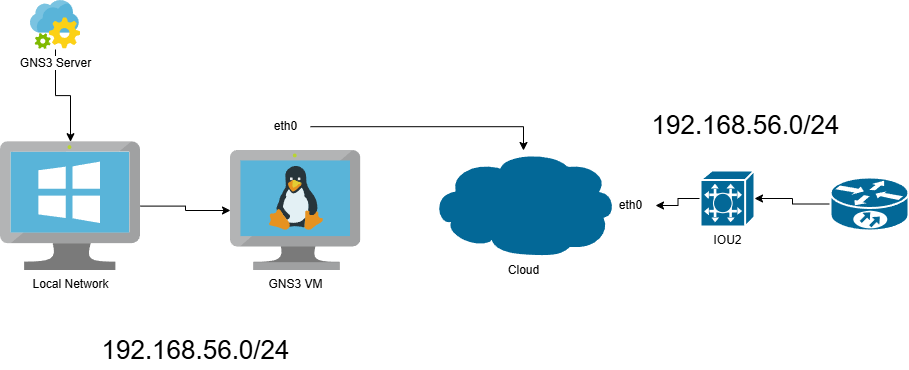
\includegraphics[width=1.1\textwidth]{graphics/network_topology_high_level.png}
	\caption{\en{Network topology design}}
\end{figure}

\FloatBarrier

\section{Οδηγός χρήσης της εφαρμογής}

\section{Εκκίνηση της εφαρμογής}

\subsection{Τοπικά}

Προκειμένου να εκκινήσουμε την εφαρμογή τοπικά ακολουθούμε τα παρακάτω βήματα:

\begin{itemize}
    \item Βρισκόμαστε στο \en{/home path}.
    \item Κατεβάζουμε την εφαρμογή με την εντολή \selectlanguage{english} git clone \url{https://github.com/Iasimo92/SDN_Django_framework_for_implementation_network_service_configuration_application}. \selectlanguage{greek}.
    \item Μπαίνουμε στο φάκελο που κατεβάσαμε. Στο φάκελο αυτό βρίσκονται τα αρχεία \en{requirements.txt} και \en{manage.py}.
    \item Τρέχουμε την εφαρμογή με την εντολή \en{python3 manage.py runserver}.

\end{itemize}

\subsection{\en{Docker Container}}

Αφού έχει φτιαχτεί το \en{image} με βάση την εντολή \en{docker build-t djangothesis:v2} όπως περιγράφηκε στην ενότητα 8.1.1 μπορούμε να τρέξουμε την εφαρμογή με την εντολή \en{docker run}. Τα βήματα που ακολουθούνται είναι τα παρακάτω:


\begin{itemize}
    \item Ελέγχουμε με την εντολή \en{docker image list} ότι έχουμε το \en{image} που θέλουμε να τρέξουμε. Αυτή η εντολή φαίνεται στην εικόνα 8.5 της ενότητας 8.1.
    \item Τρέχουμε το \en{container} με την εντολή \en{ docker run -d -p 8000:8000 --name djangothesis\_container djangothesis:v2.}
    \item Η εφαρμογή τώρα είναι διαθέσιμη στο \en{browser} μας.

\end{itemize}

\subsection{\en{Access} της εφαρμογής μέσα από το \en{pod}}

Ο συγκεκριμένος τρόπος εξηγείται αναλυτικά στην ενότητα 8.2.2.

\subsection{Δημιουργία αντικειμένου-Προσθήκη συσκευής}

Προκειμένου να μπορούμε να διαχειριστούμε συσκευή θα πρέπει να την εισάγουμε ως αντικείμενο.

Ανοίγουμε το \en{http://127.0.0.1:8000/admin/} σε \en{browser} και εισάγουμε ως χρήστη \en{iasonas}
και κωδικό \en{ericsson}.

\FloatBarrier

\begin{figure}[h]
	\centering
	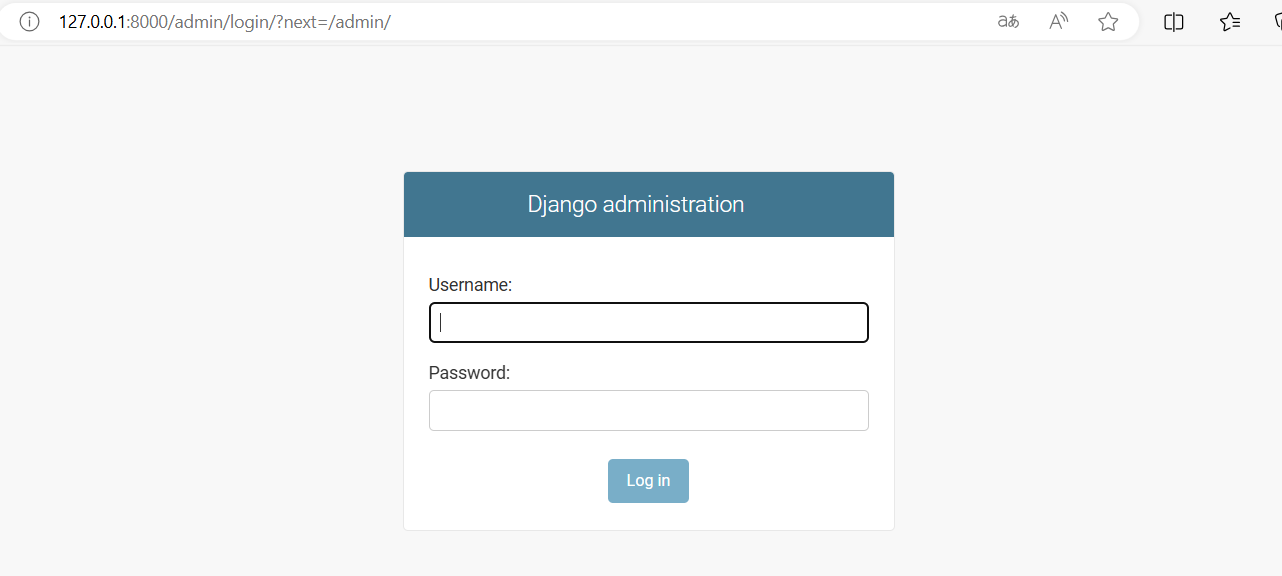
\includegraphics[width=1.1\textwidth]{graphics/GUI_LOGIN.png}
	\caption{\en{GUI Login}}
\end{figure}

\FloatBarrier

Αφού συνδεθούμε στο \en{GUI} επιλέγουμε \en{Network}, \en{Devices} και \en{Add} προκειμένου να εισάγουμε καινούργια συσκευή.

\FloatBarrier

\begin{figure}[h]
	\centering
	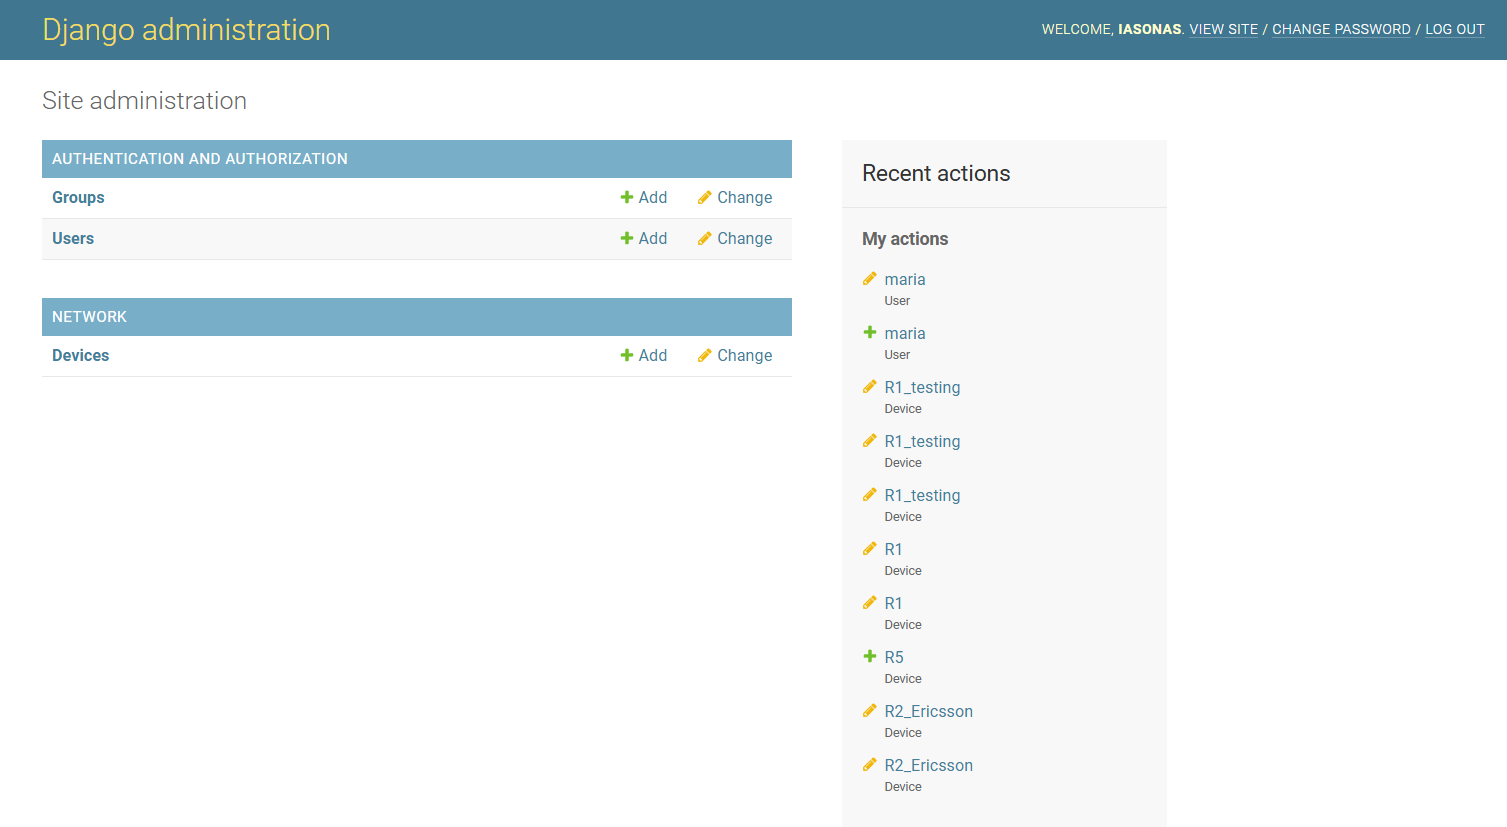
\includegraphics[width=1.1\textwidth]{graphics/DJANGO_ADMIN.png}
	\caption{\en{GUI Login second page}}
\end{figure}

\FloatBarrier

Στη συνέχεια μας εμφανίζεται η παρακάτω εικόνα. Βάζουμε τα στοιχεία της συσκευής και πατάμε αποθήκευση.

\FloatBarrier

\begin{figure}[h]
	\centering
	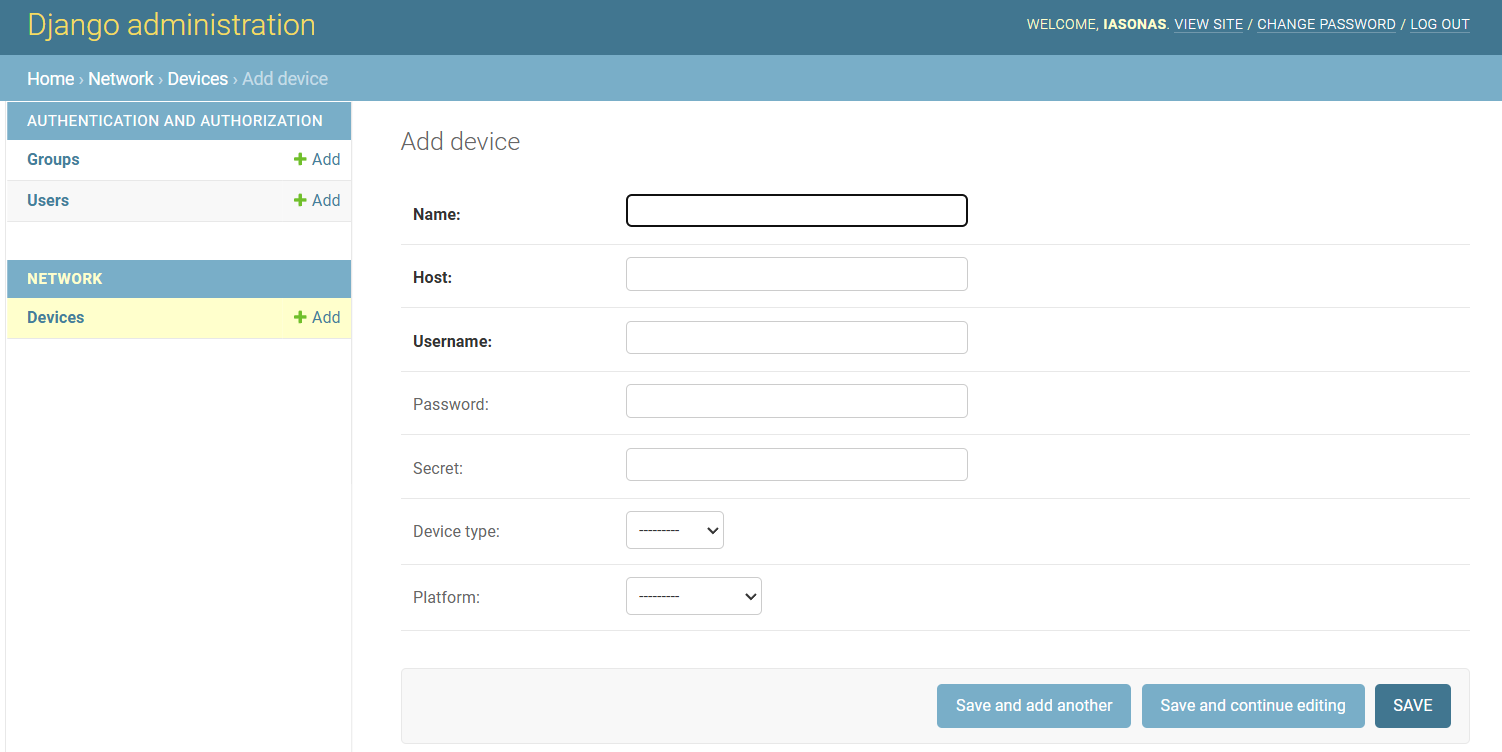
\includegraphics[width=1.1\textwidth]{graphics/ADD_DEVICE.png}
	\caption{\en{Add device page}}
\end{figure}

\FloatBarrier

Αφού το κάνουμε αυτό όλες οι συσκευές που προσθέσαμε μπορούμε να τις δούμε σε όλες τις λειτουργίες της εφαρμογής.
Οι λειτουργίες μπορούν να εκτελεστούν μια μια όπως έγινε στο \en{application demo}.

\section{Κώδικας}

H εφαρμογή είναι ελεύθερη στη σελίδα: \selectlanguage{english} \url{https://github.com/Iasimo92/SDN_Django_framework_for_implementation_network_service_configuration_application}. \selectlanguage{greek}


\FloatBarrier

\begin{figure}[h]
	\centering
	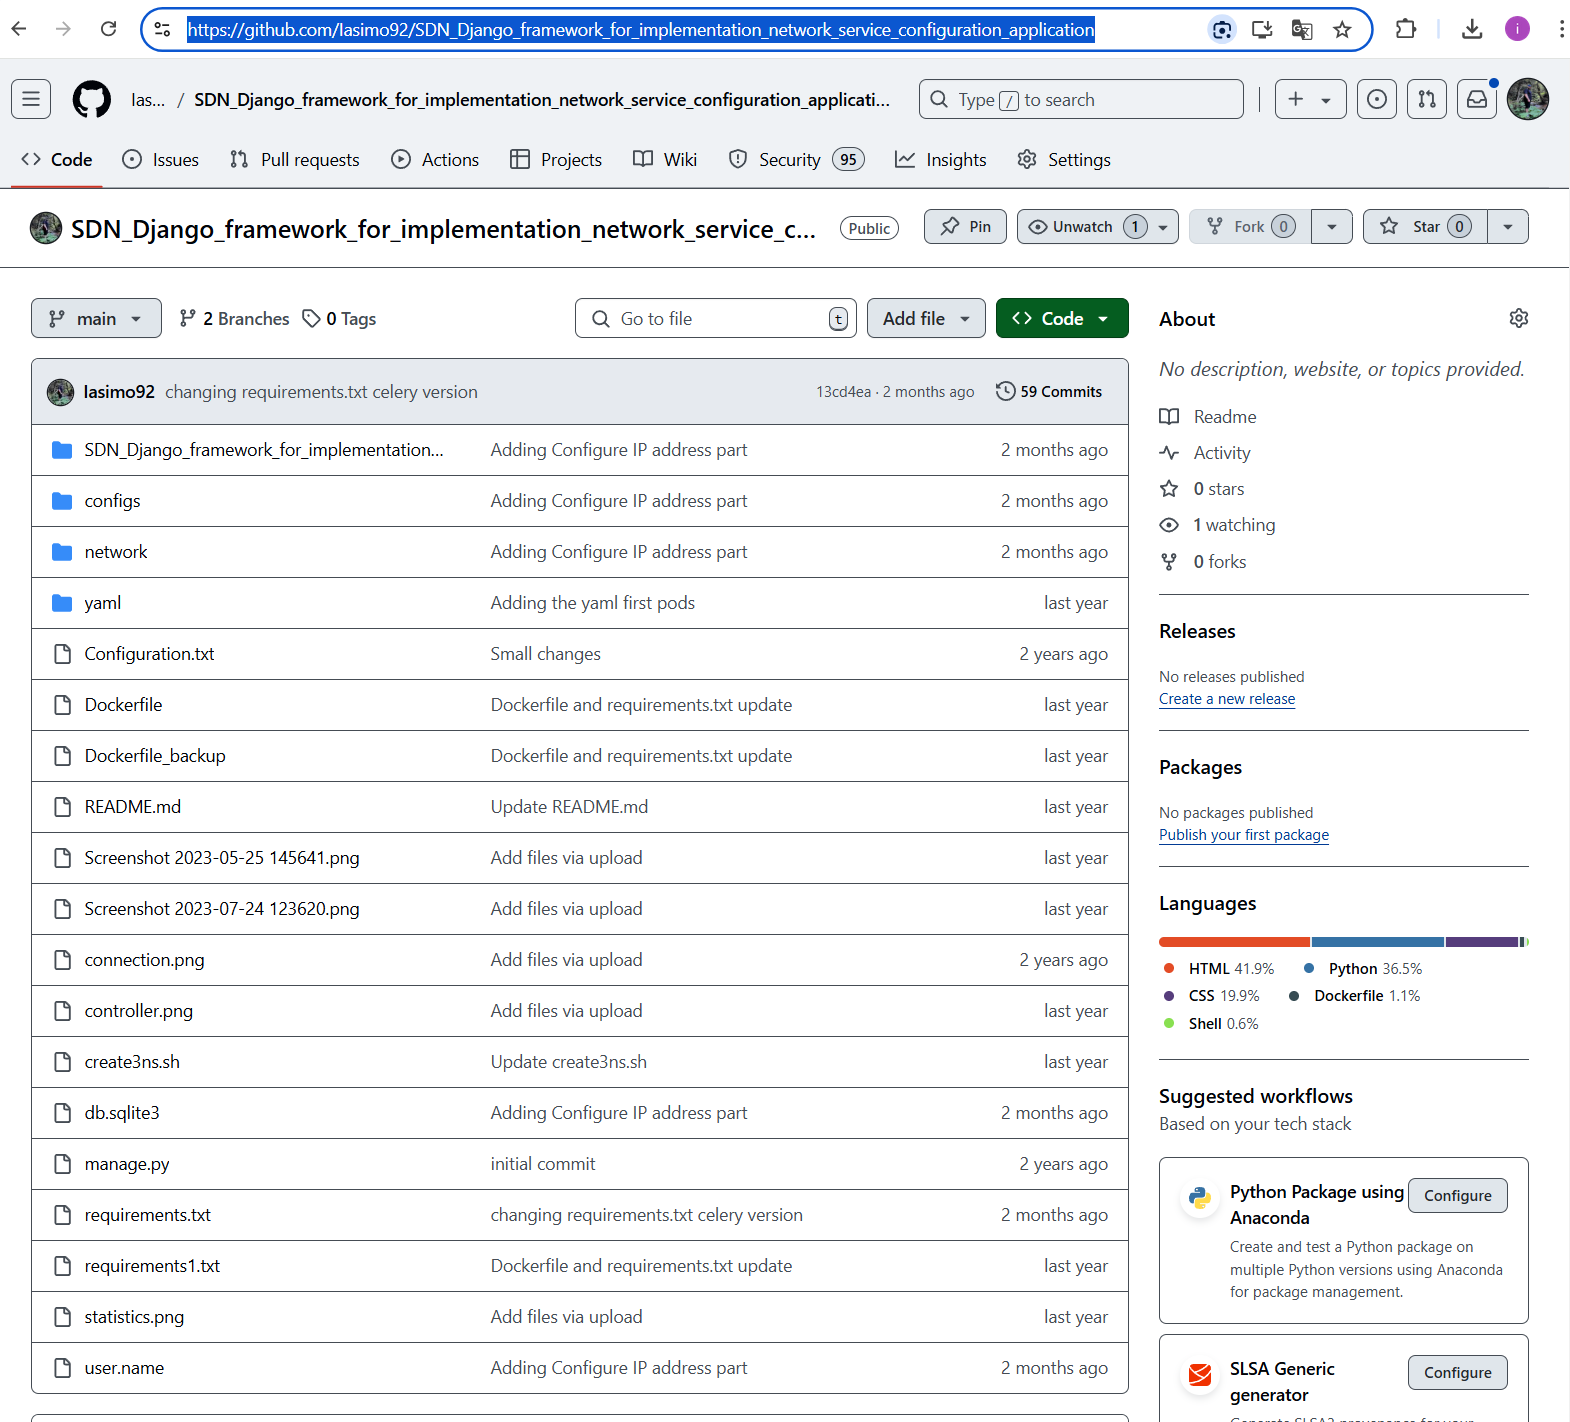
\includegraphics[width=1.1\textwidth]{graphics/github_page.png}
	\caption{\en{github repo}}
\end{figure}

\FloatBarrier

